% Options for packages loaded elsewhere
\PassOptionsToPackage{unicode}{hyperref}
\PassOptionsToPackage{hyphens}{url}
\PassOptionsToPackage{dvipsnames,svgnames,x11names}{xcolor}
\documentclass[
  10pt,
]{article}
\usepackage{xcolor}
\usepackage[margin=2cm]{geometry}
\usepackage{amsmath,amssymb}
\setcounter{secnumdepth}{5}
\usepackage{iftex}
\ifPDFTeX
  \usepackage[T1]{fontenc}
  \usepackage[utf8]{inputenc}
  \usepackage{textcomp} % provide euro and other symbols
\else % if luatex or xetex
  \usepackage{unicode-math} % this also loads fontspec
  \defaultfontfeatures{Scale=MatchLowercase}
  \defaultfontfeatures[\rmfamily]{Ligatures=TeX,Scale=1}
\fi
\usepackage{lmodern}
\ifPDFTeX\else
  % xetex/luatex font selection
  \setmainfont[]{Latin Modern Roman}
\fi
% Use upquote if available, for straight quotes in verbatim environments
\IfFileExists{upquote.sty}{\usepackage{upquote}}{}
\IfFileExists{microtype.sty}{% use microtype if available
  \usepackage[]{microtype}
  \UseMicrotypeSet[protrusion]{basicmath} % disable protrusion for tt fonts
}{}
\makeatletter
\@ifundefined{KOMAClassName}{% if non-KOMA class
  \IfFileExists{parskip.sty}{%
    \usepackage{parskip}
  }{% else
    \setlength{\parindent}{0pt}
    \setlength{\parskip}{6pt plus 2pt minus 1pt}}
}{% if KOMA class
  \KOMAoptions{parskip=half}}
\makeatother
\usepackage{longtable,booktabs,array}
\newcounter{none} % for unnumbered tables
\usepackage{calc} % for calculating minipage widths
% Correct order of tables after \paragraph or \subparagraph
\usepackage{etoolbox}
\makeatletter
\patchcmd\longtable{\par}{\if@noskipsec\mbox{}\fi\par}{}{}
\makeatother
% Allow footnotes in longtable head/foot
\IfFileExists{footnotehyper.sty}{\usepackage{footnotehyper}}{\usepackage{footnote}}
\makesavenoteenv{longtable}
\usepackage{graphicx}
\makeatletter
\newsavebox\pandoc@box
\newcommand*\pandocbounded[1]{% scales image to fit in text height/width
  \sbox\pandoc@box{#1}%
  \Gscale@div\@tempa{\textheight}{\dimexpr\ht\pandoc@box+\dp\pandoc@box\relax}%
  \Gscale@div\@tempb{\linewidth}{\wd\pandoc@box}%
  \ifdim\@tempb\p@<\@tempa\p@\let\@tempa\@tempb\fi% select the smaller of both
  \ifdim\@tempa\p@<\p@\scalebox{\@tempa}{\usebox\pandoc@box}%
  \else\usebox{\pandoc@box}%
  \fi%
}
% Set default figure placement to htbp
\def\fps@figure{htbp}
\makeatother
\setlength{\emergencystretch}{3em} % prevent overfull lines
\providecommand{\tightlist}{%
  \setlength{\itemsep}{0pt}\setlength{\parskip}{0pt}}
% Keep each figure where the text puts it, and let long code paths break.
\usepackage{float}
\floatplacement{figure}{H}
\usepackage{etoolbox}
\AtBeginEnvironment{longtable}{\small}
\sloppy
\usepackage{bookmark}
\IfFileExists{xurl.sty}{\usepackage{xurl}}{} % add URL line breaks if available
\urlstyle{same}
\hypersetup{
  pdftitle={hwde-led-test: board report},
  colorlinks=true,
  linkcolor={Maroon},
  filecolor={Maroon},
  citecolor={Blue},
  urlcolor={Blue},
  pdfcreator={LaTeX via pandoc}}

\title{hwde-led-test: board report}
\usepackage{etoolbox}
\makeatletter
\providecommand{\subtitle}[1]{% add subtitle to \maketitle
  \apptocmd{\@title}{\par {\large #1 \par}}{}{}
}
\makeatother
\subtitle{The first board the Hive designed with the hwde module}
\author{}
\date{2026-10-28}

\begin{document}
\maketitle

{
\setcounter{tocdepth}{3}
\tableofcontents
}
\section{What this is}\label{what-this-is}

This report covers \textbf{hwde-led-test}, a tiny 2-layer board that
lights one green LED from 5 V. It was the first board the Hive designed
end to end with the hive-hwde module, on 2026-10-28. It went from a
written brief to checked fab files in about 45 minutes, to prove the
pipeline runs inside the Hive. \textbf{It has not been ordered or
quoted.} Ordering is your call.

The run went on through the stages while three sign-offs were still
waiting for your answer: H1 (architecture), H2 (schematic) and H4
(verified board). H4 also asks you to waive two verify warnings. Those
five decisions are in \hyperref[decisions-waiting-for-you]{section 8},
each with what it asks and a recommended answer. This report puts
everything you need for them in one place.

{\def\LTcaptype{none} % do not increment counter
\begin{longtable}[]{@{}
  >{\raggedright\arraybackslash}p{(\linewidth - 2\tabcolsep) * \real{0.1429}}
  >{\raggedright\arraybackslash}p{(\linewidth - 2\tabcolsep) * \real{0.8571}}@{}}
\toprule\noalign{}
\endhead
\bottomrule\noalign{}
\endlastfoot
Board & 2 layers, 1.6 mm FR-4, 1 oz, HASL (JLC2313), 13.4 x 10.5 mm, no
holes \\
Circuit & J1 5 V header, C1 4.7 µF input cap, R1 470 Ω, D1 green 0603
LED (about 4 mA) \\
Gates & ERC, place, routed DRC, verify (14 checks), JLC DFM: \textbf{all
pass} \\
Open & 2 verify warnings not waived; H1, H2 and H4 not answered \\
Parts cost & about \$0.05 a board at LCSC single-piece prices (JLC fees
not quoted) \\
Run time & about 45 minutes, brief to DFM-clean package; 9 subagents,
325k tokens \\
\end{longtable}
}

\begin{figure}
\centering
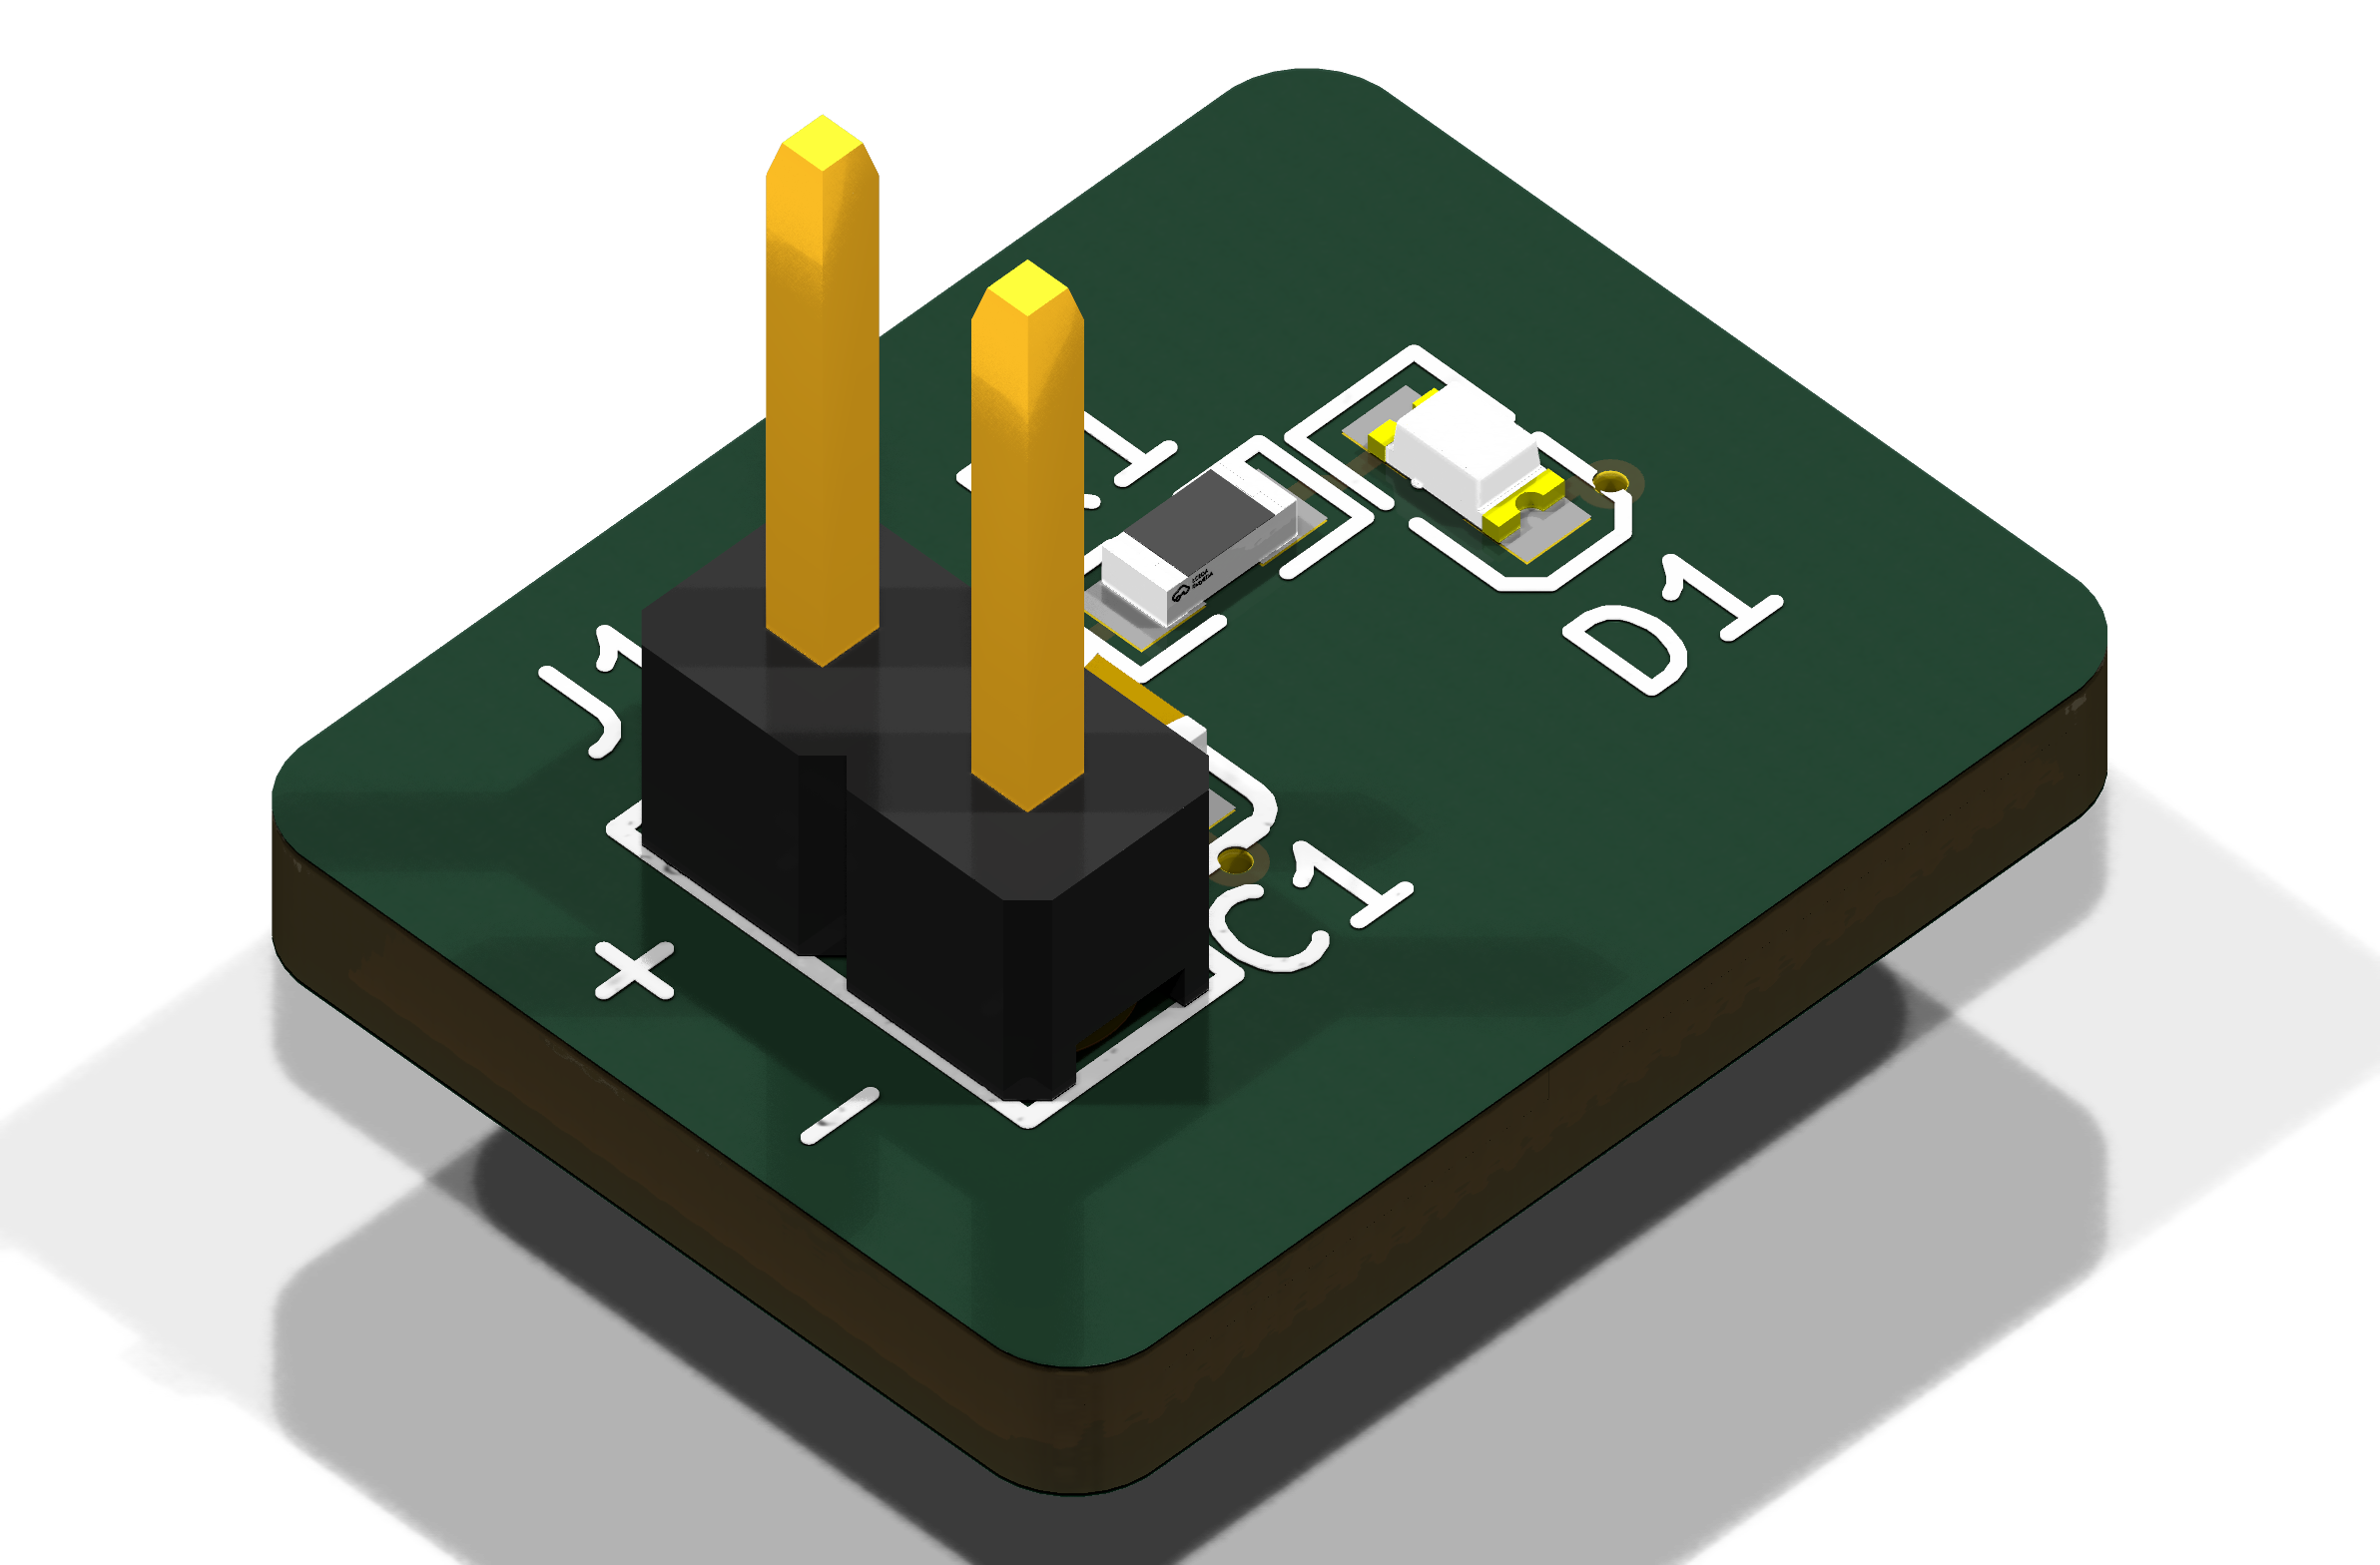
\includegraphics[width=0.85\linewidth,height=\textheight,keepaspectratio,alt={The board, 3D render (iso)}]{img/hwde-led-test_iso.png}
\caption{The board, 3D render (iso)}
\end{figure}

\section{What the board is}\label{what-the-board-is}

The brief asked for ``a tiny 2-layer board that lights one LED from 5
V'':

\begin{itemize}
\tightlist
\item
  \textbf{Input:} 5 V DC (4.75--5.25 V) on J1, a 2-pin 2.54 mm header.
  Pin 1 is +5V (square pad, marked \textbf{+}) and pin 2 is GND (marked
  \textbf{−}). It is fed from a bench supply or a USB 5 V lead. As the
  brief asked, there is no reverse-polarity protection.
\item
  \textbf{C1:} 4.7 µF 16 V X5R 0603 across the input, next to J1.
\item
  \textbf{R1 + D1:} 470 Ω feeds a green 0603 LED (KT-0603G). At the
  LED's listed forward voltage of 3.1 V, that gives 3.5 mA at 4.75 V,
  4.0 mA at 5.0 V and 4.6 mA at 5.25 V, inside the brief's 3--5 mA.
\item
  \textbf{Layout:} all SMD parts are on top. J1 is through-hole on the
  left edge, and the bottom layer is a GND pour.
\item
  \textbf{Built:} 5 boards if it is ever built. It is meant for room
  temperature on a bench, with no enclosure.
\end{itemize}

\section{Schematic}\label{schematic}

There is one sheet with four parts and three nets: +5V, GND and LED\_A.
ERC reports 0 errors and 0 warnings, and a fresh-context reviewer found
0 errors (\texttt{reports/review-schematic.md}). The full sheet is
\texttt{reports/schematic.pdf}. Below is the drawn area, cropped from
that sheet.

\begin{figure}
\centering
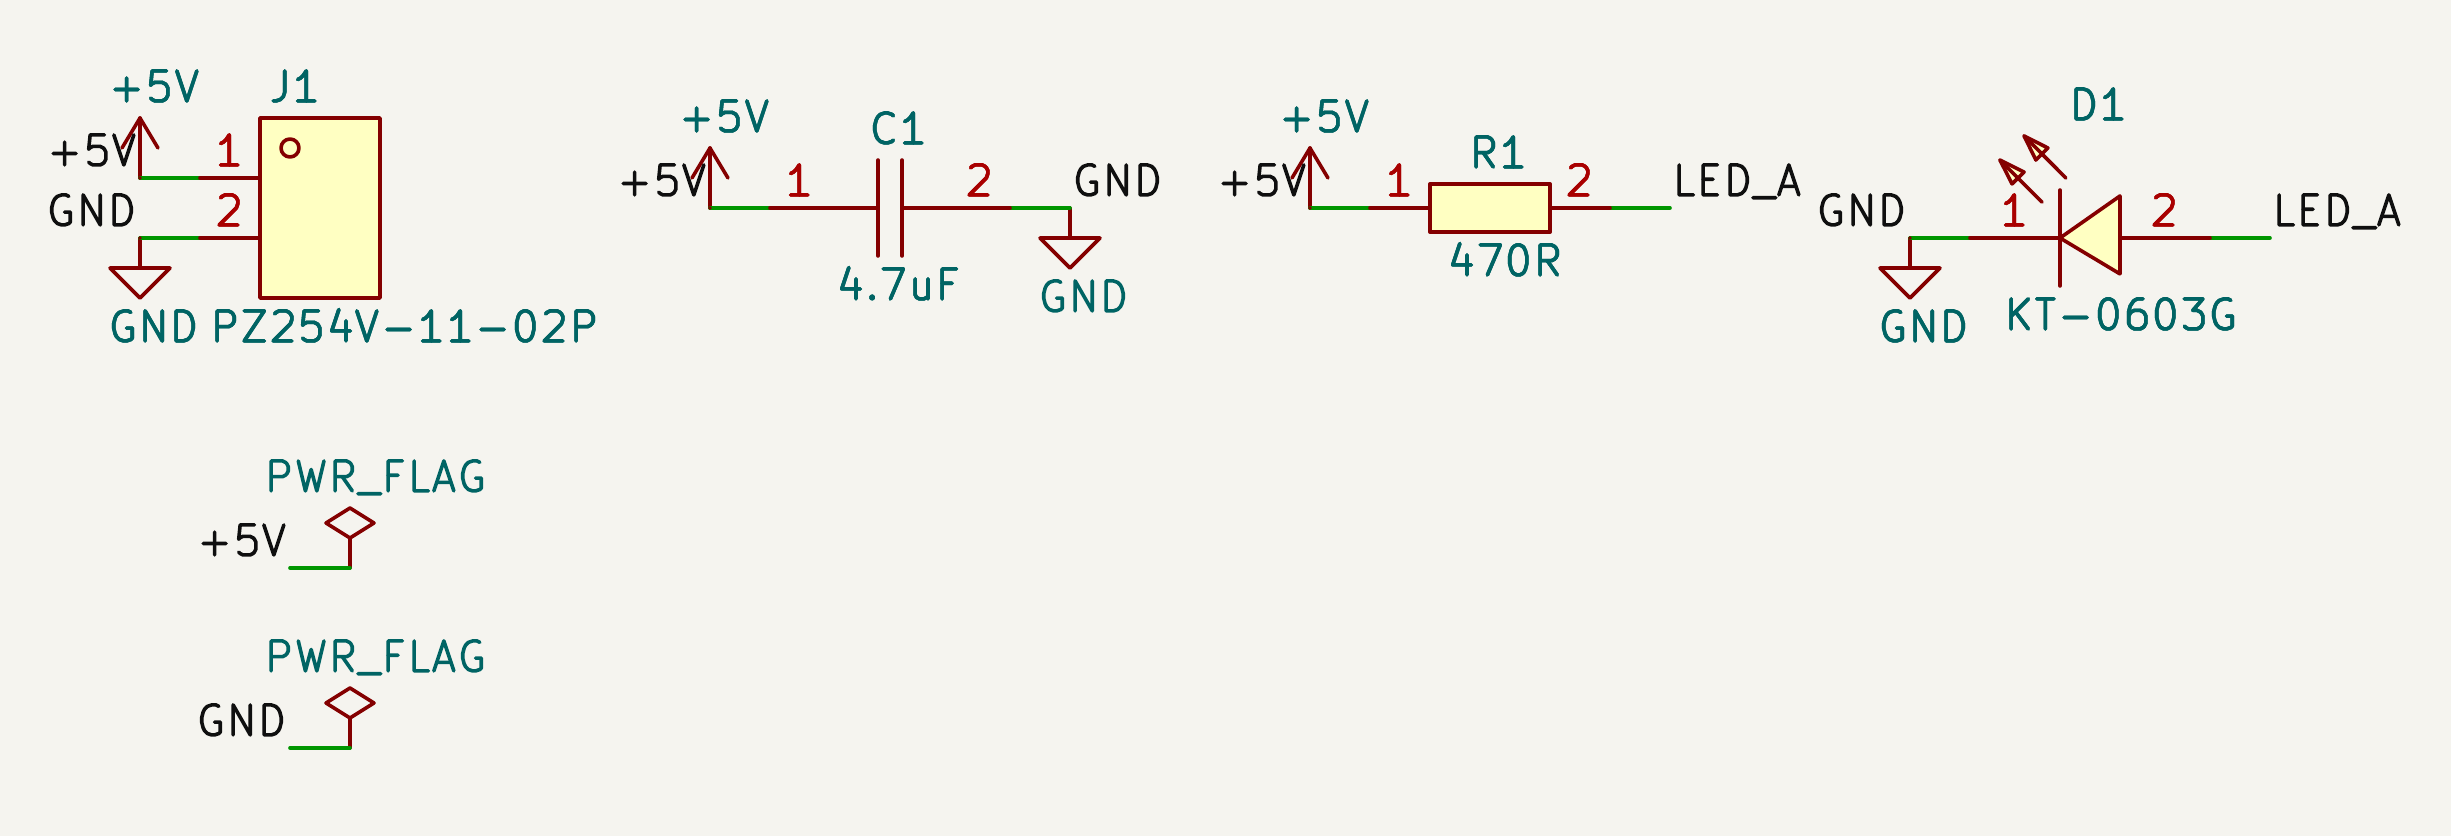
\includegraphics[width=1\linewidth,height=\textheight,keepaspectratio,alt={Schematic (cropped from reports/schematic.pdf)}]{img/hwde-led-test_schematic.png}
\caption{Schematic (cropped from reports/schematic.pdf)}
\end{figure}

The generator first drew this sheet poorly: each net label sat on its
pin number (``+5V'' ran into ``1''), the circuit was small in one corner
of an A4 sheet, and D1's ``K'' and ``A'' pin names printed over each
other (\hyperref[snags-the-run-hit]{snag 14}). \texttt{schlib} now turns
every label away from its pin, hides the pin names of two-pin parts, and
sizes the paper to the drawing (A5 here) with the drawing centred on it.
The netlist and the symbols' UUIDs didn't change.

\section{Layout}\label{layout}

The board is 13.4 x 10.5 mm, with 2.0 mm corner radii. All four parts
sit on the top side in one row: J1 on the left edge, C1 beside it, then
R1 and D1. +5V runs from J1 pin 1 through C1's pad to R1. LED\_A runs
from R1 to D1's anode. C1's GND and D1's cathode each drop through their
own via to the bottom GND pour, and J1 pin 2 is thermal-tied to that
pour.

The two copper layer views below were made by the module's
\texttt{layer\_views} from the final routed board. Net names are drawn
on the copper, and both layers are seen from the top. The vector PDFs,
which stay sharp when zoomed, are \texttt{img/hwde-led-test\_F\_Cu.pdf}
and \texttt{img/hwde-led-test\_B\_Cu.pdf}.

\begin{figure}
\centering
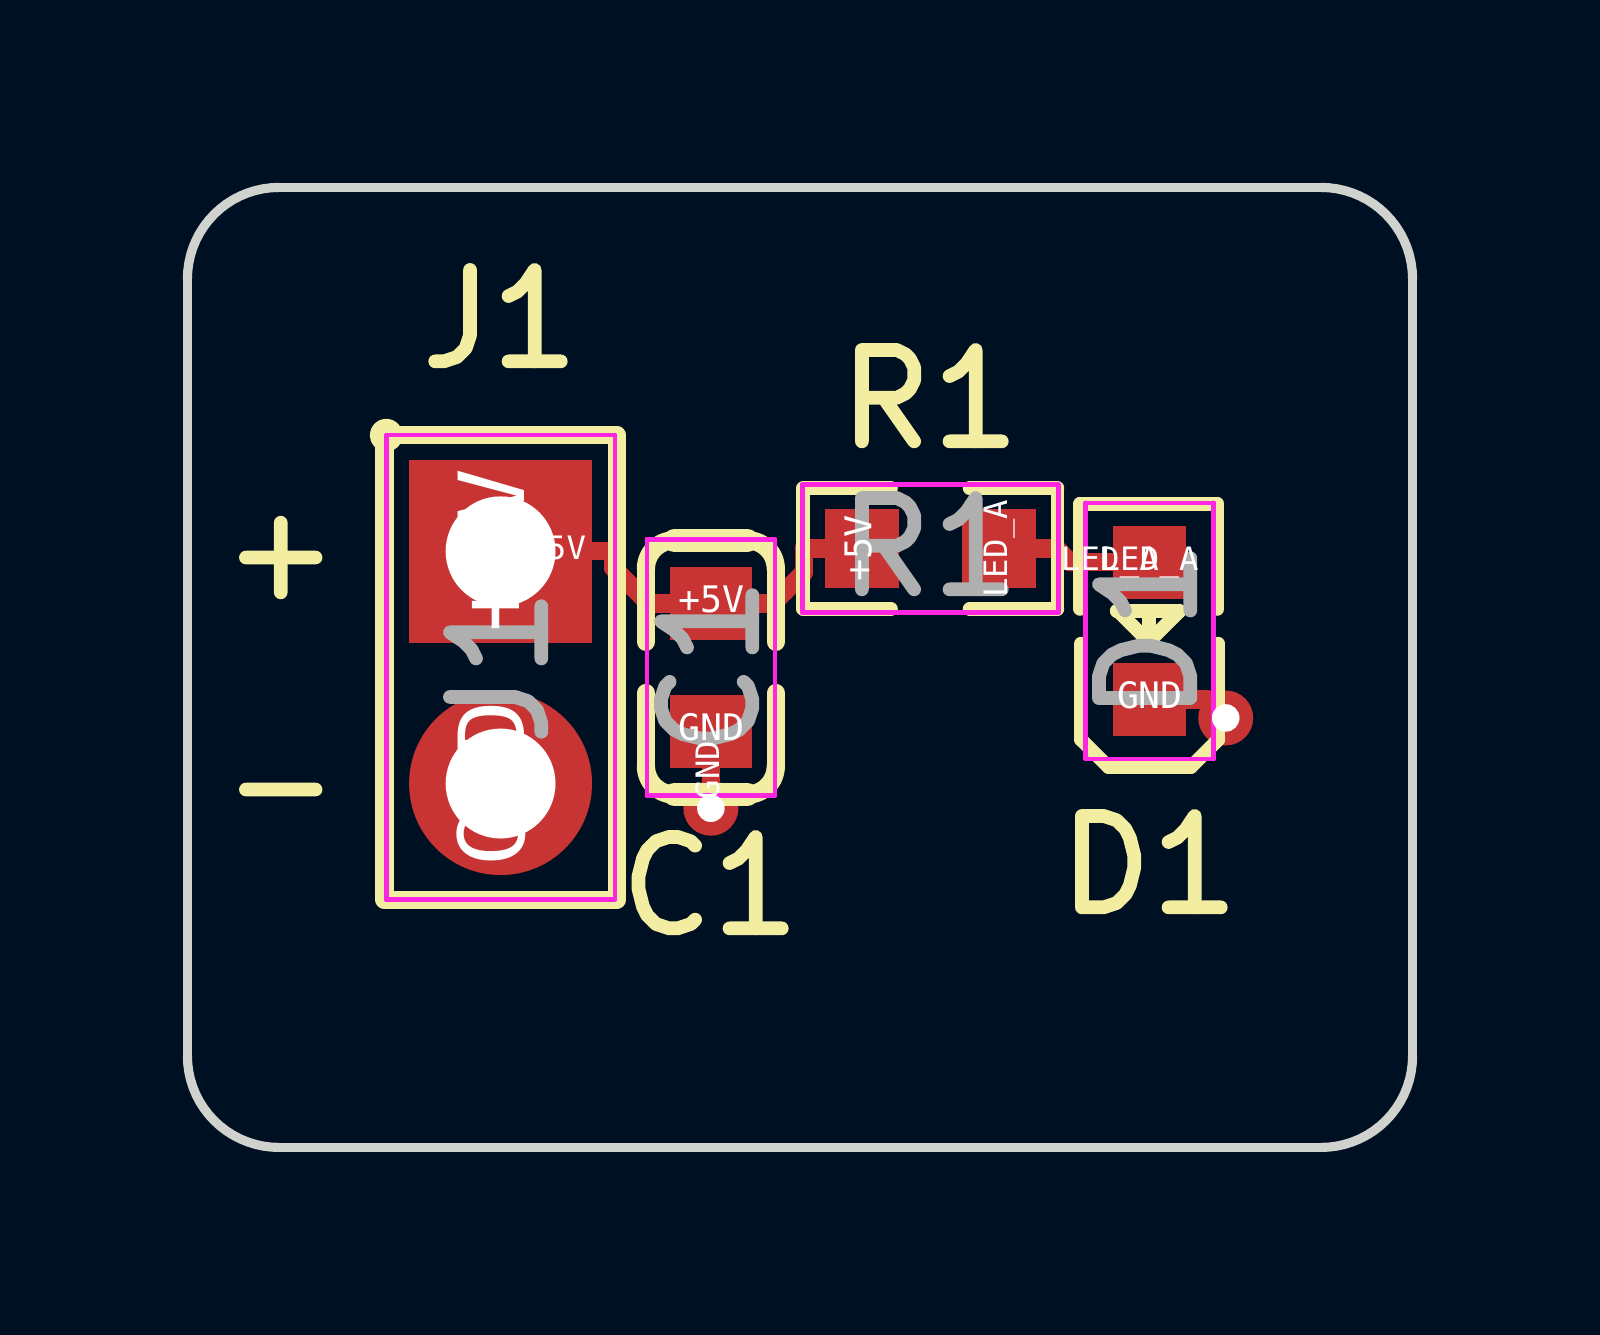
\includegraphics[width=0.62\linewidth,height=\textheight,keepaspectratio,alt={Top copper (F.Cu), with top silk, fab and courtyard}]{img/hwde-led-test_F_Cu.png}
\caption{Top copper (F.Cu), with top silk, fab and courtyard}
\end{figure}

\begin{figure}
\centering
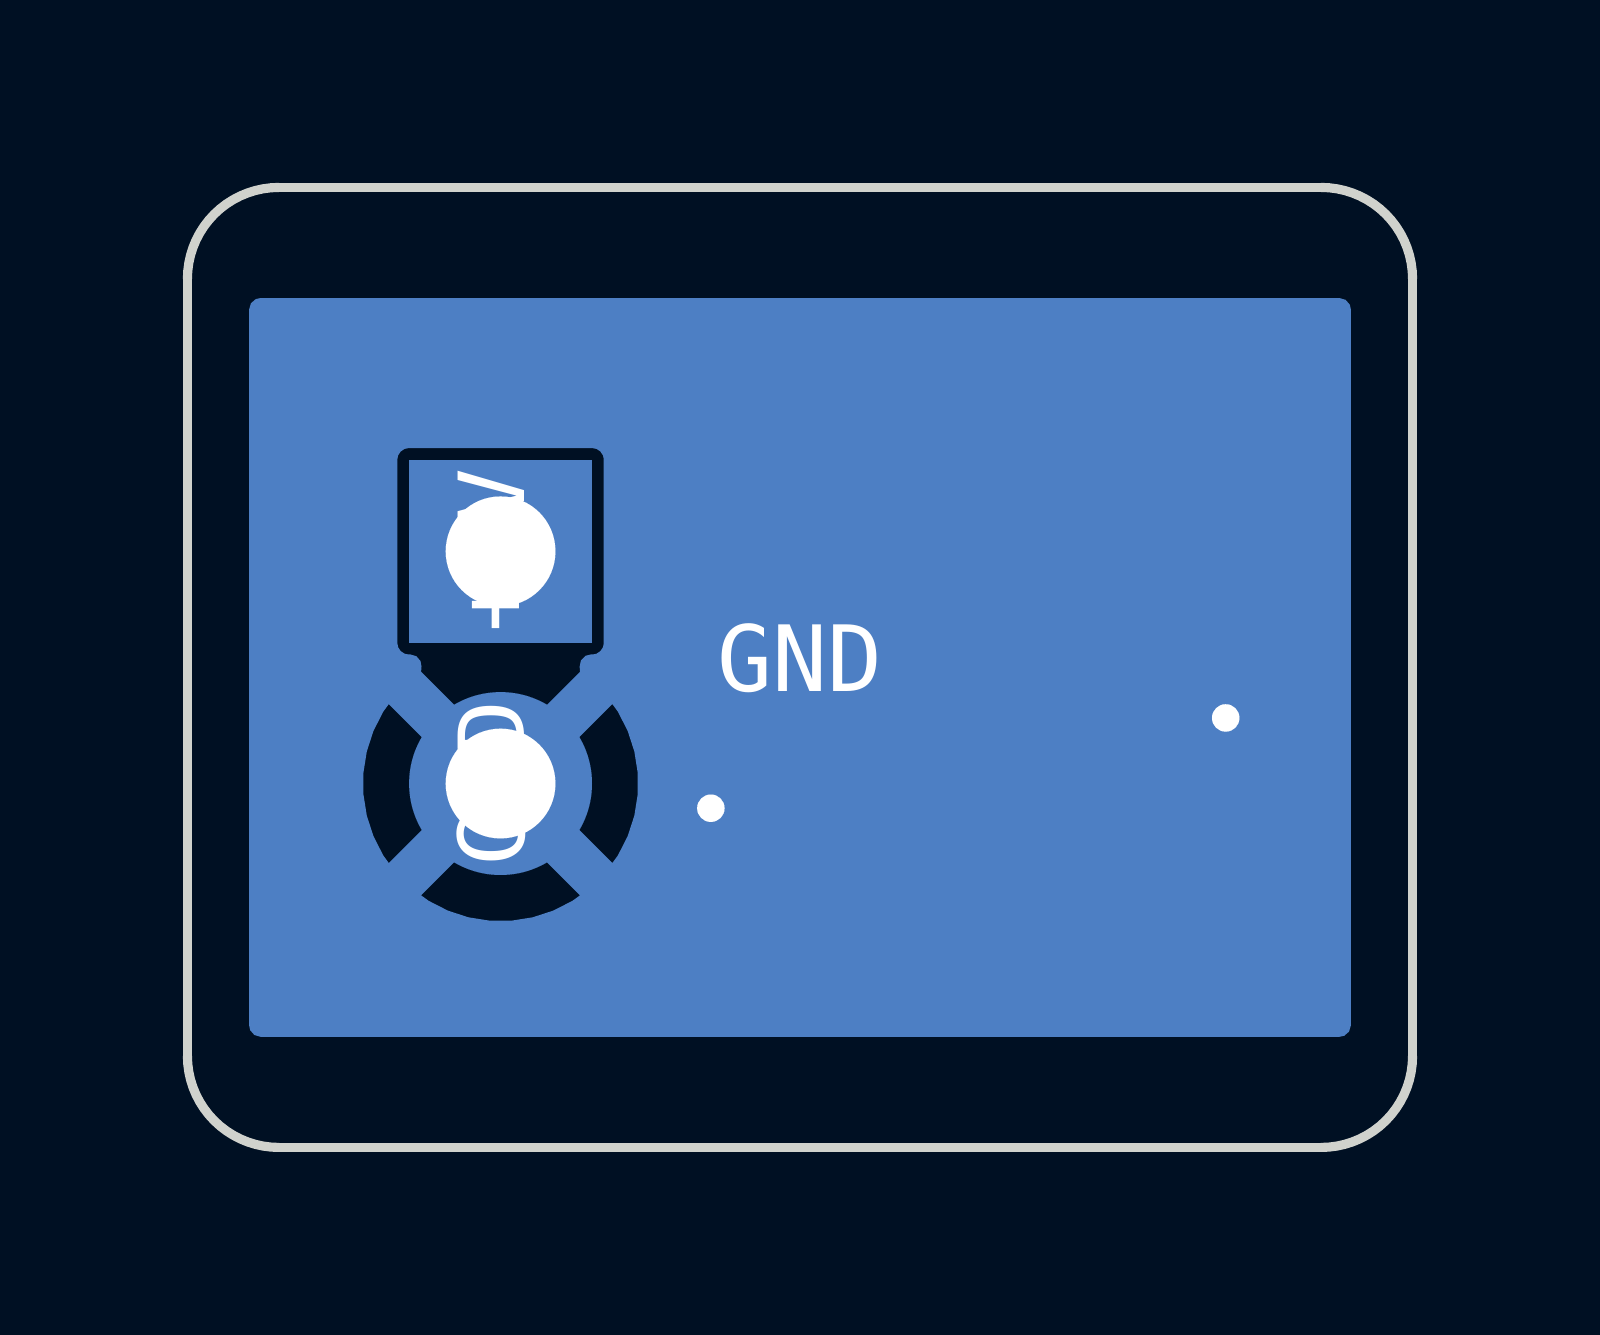
\includegraphics[width=0.62\linewidth,height=\textheight,keepaspectratio,alt={Bottom copper (B.Cu): the GND pour, seen from the top}]{img/hwde-led-test_B_Cu.png}
\caption{Bottom copper (B.Cu): the GND pour, seen from the top}
\end{figure}

The 3D renders come from KiCad 10.0.6, with the parts' EasyEDA 3D models
pulled fresh for this report:

\begin{figure}
\centering
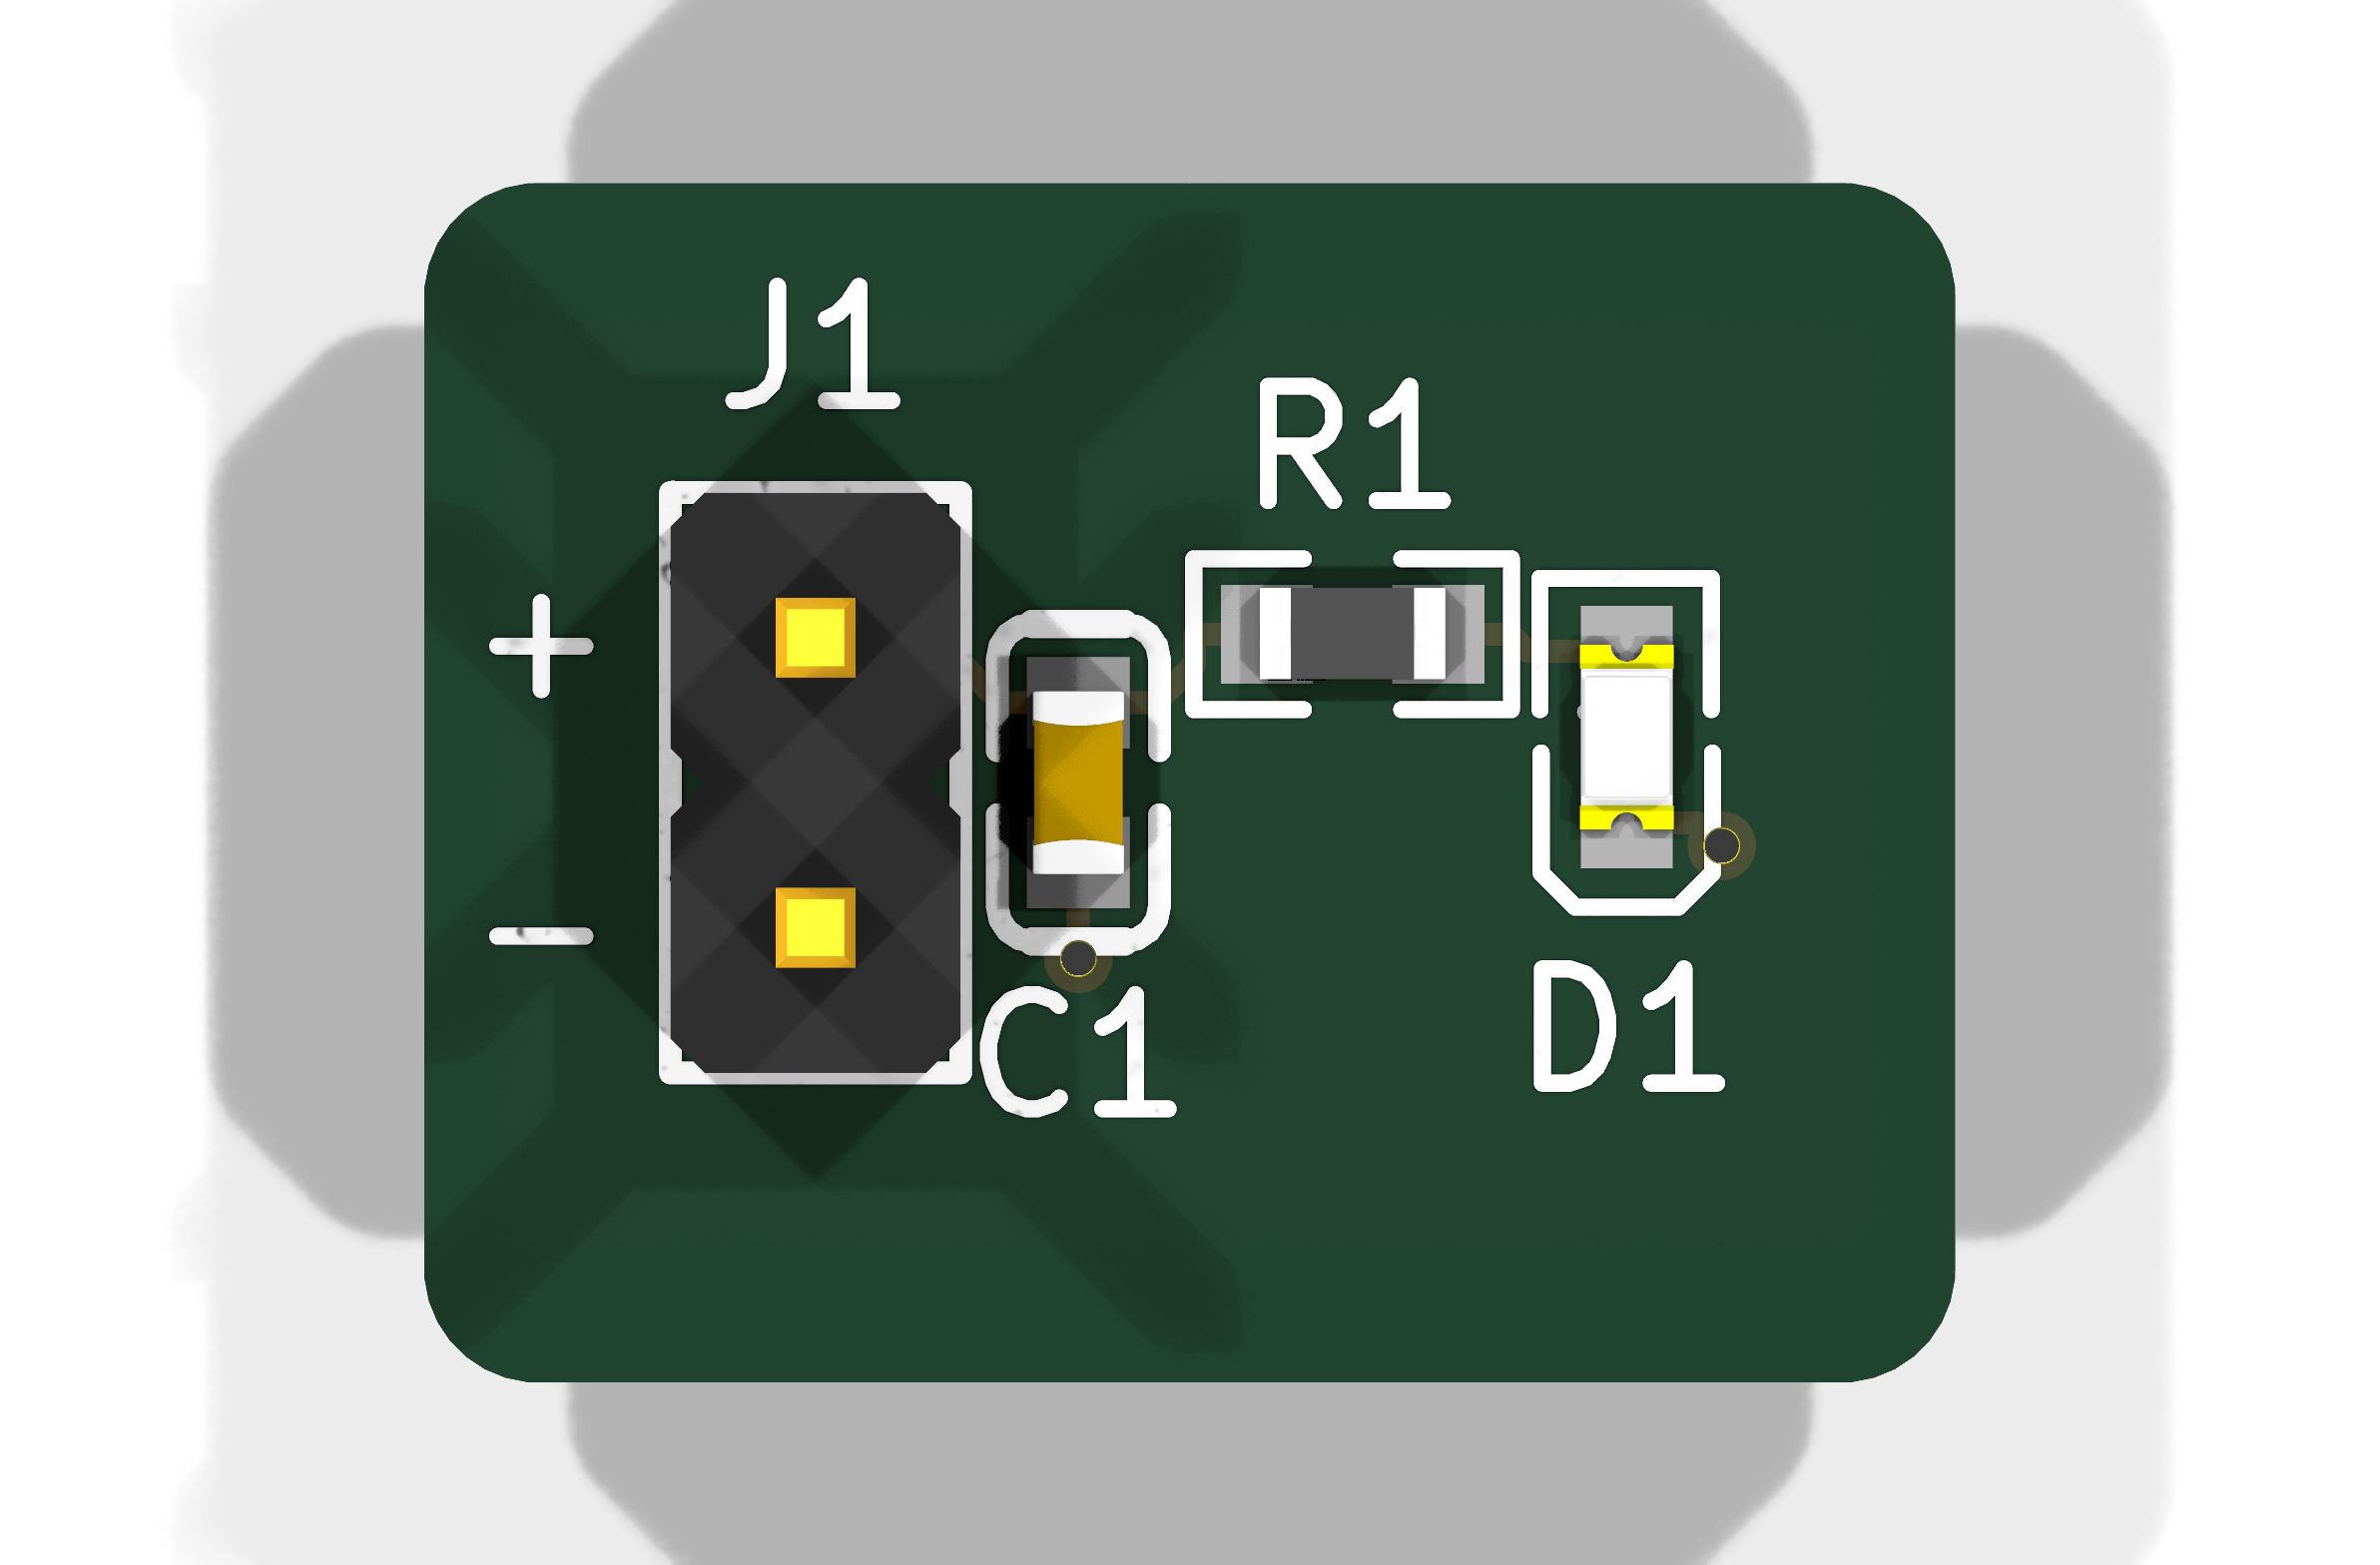
\includegraphics[width=0.85\linewidth,height=\textheight,keepaspectratio,alt={Top}]{img/hwde-led-test_top.png}
\caption{Top}
\end{figure}

\begin{figure}
\centering
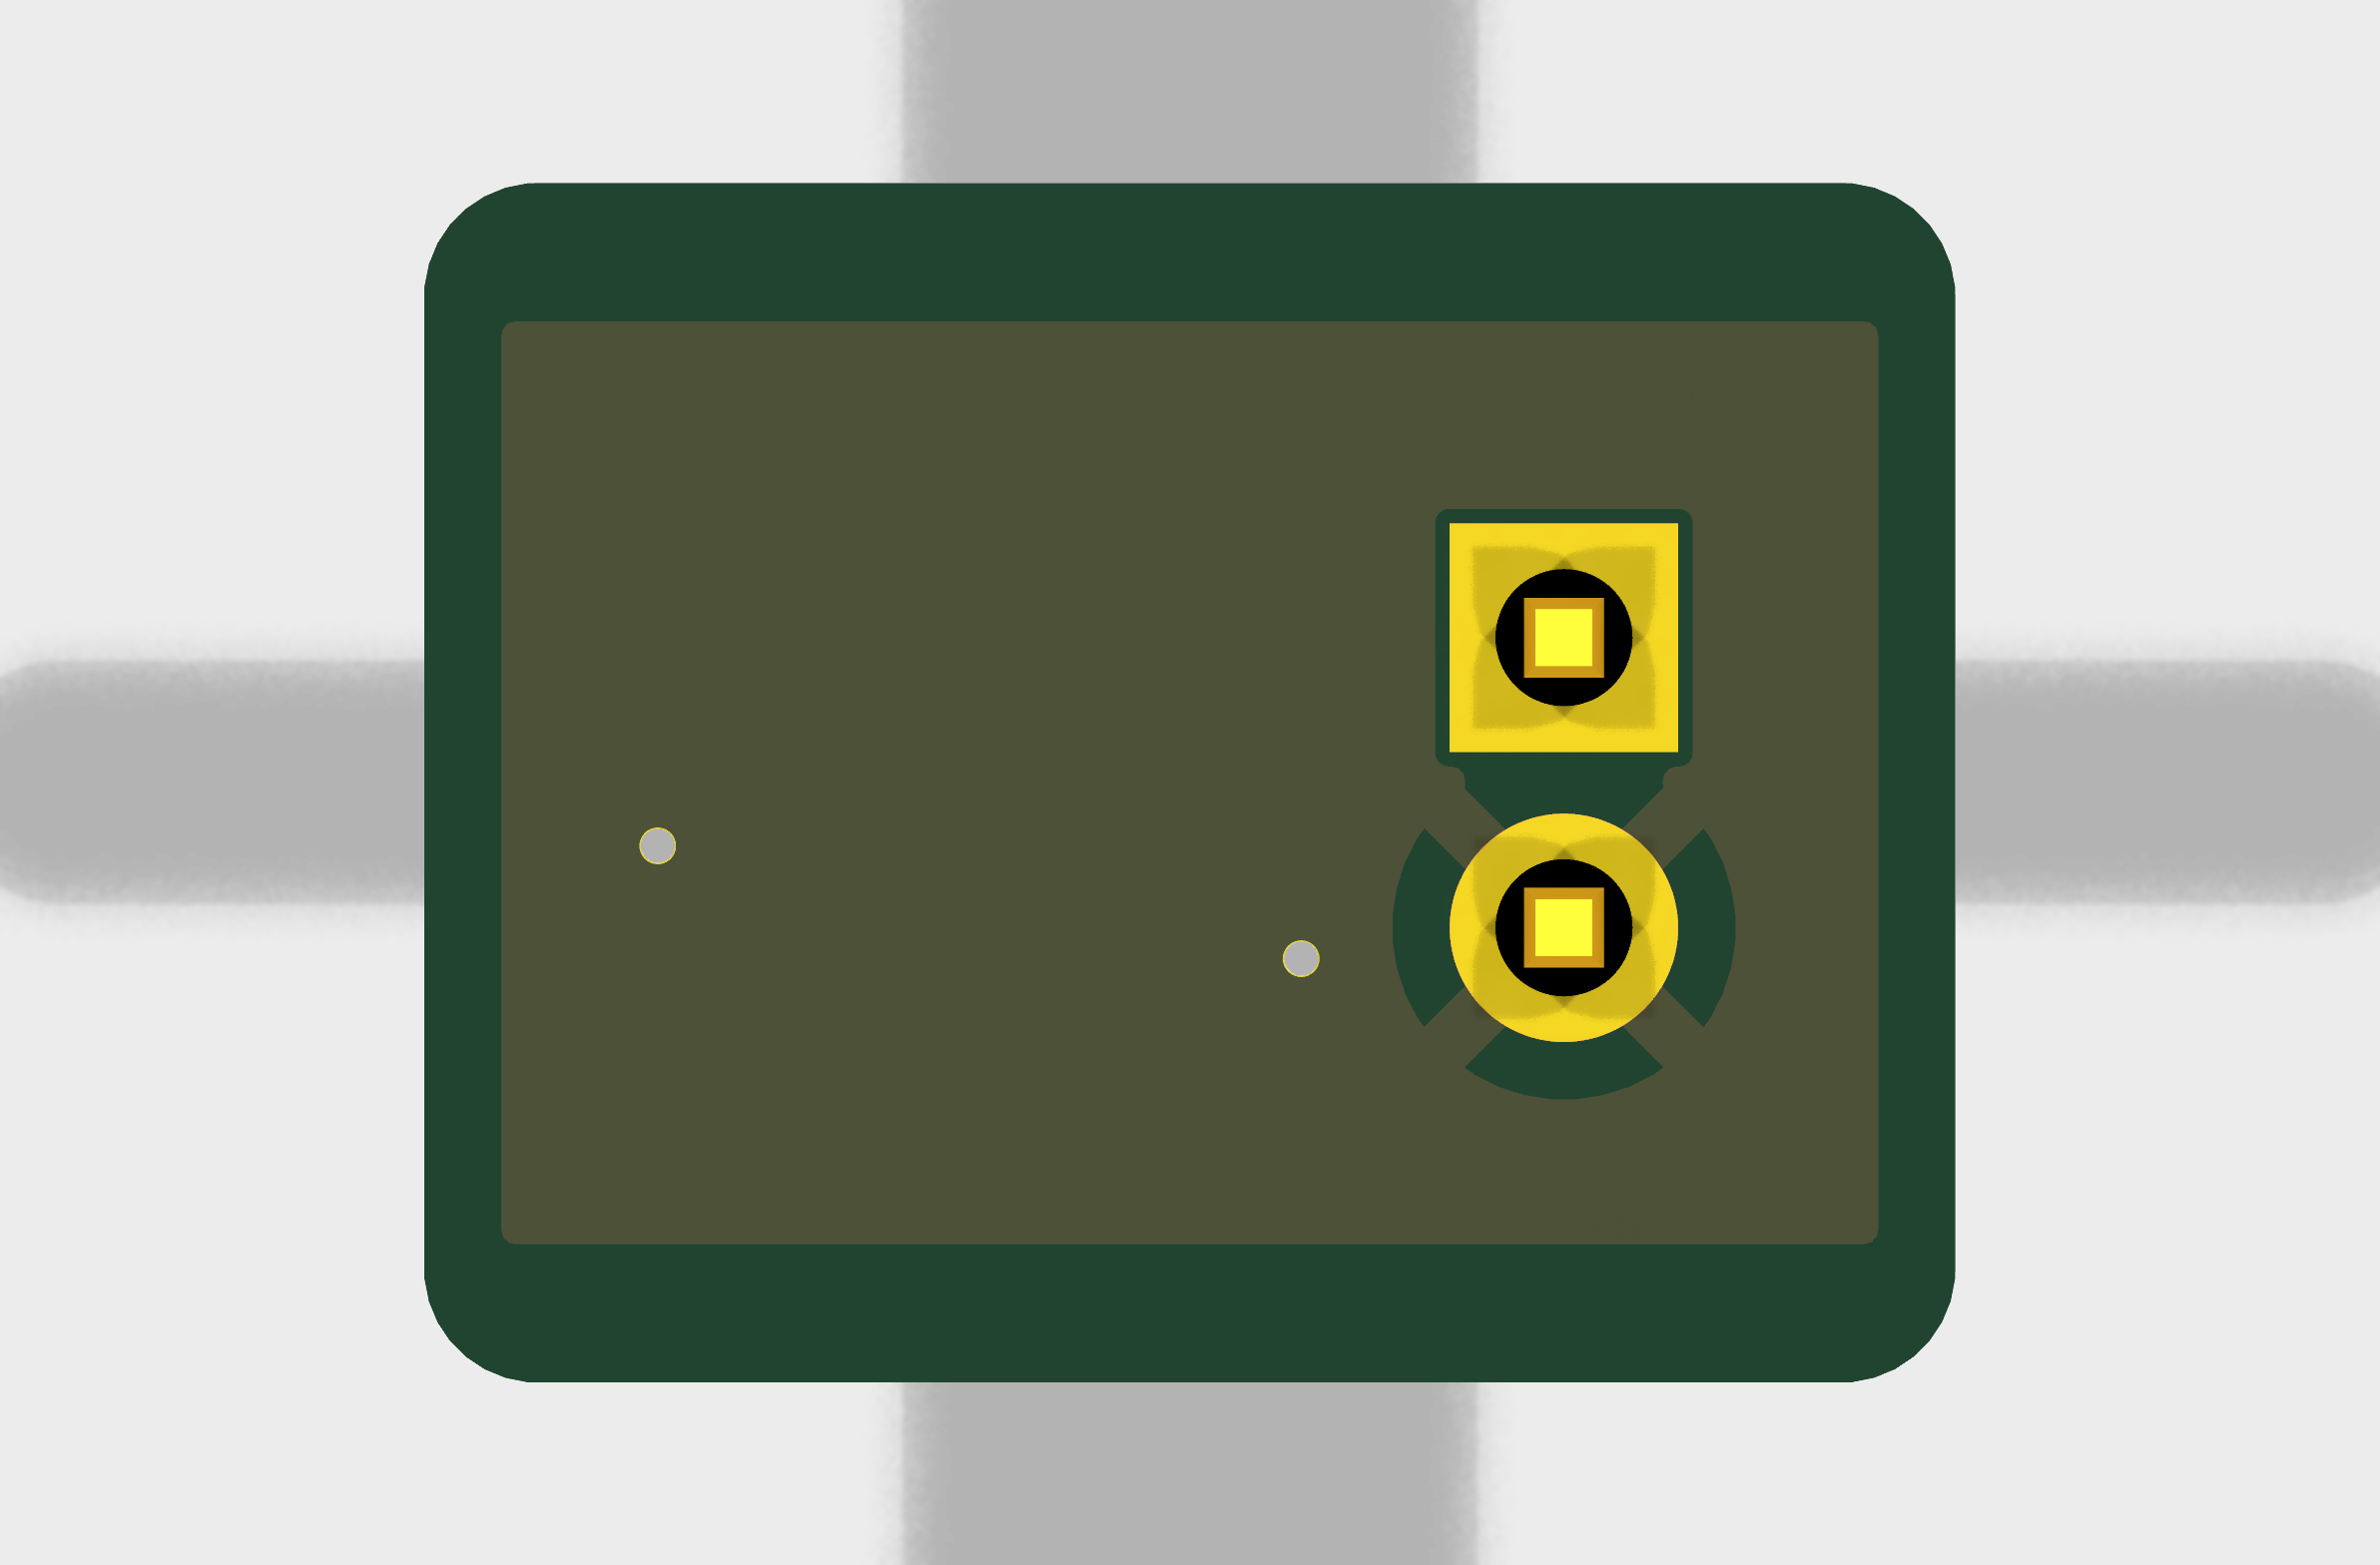
\includegraphics[width=0.85\linewidth,height=\textheight,keepaspectratio,alt={Bottom: J1's two through-hole pads, the GND pour and the two GND vias}]{img/hwde-led-test_bottom.png}
\caption{Bottom: J1's two through-hole pads, the GND pour and the two
GND vias}
\end{figure}

\section{BOM and cost}\label{bom-and-cost}

{\def\LTcaptype{none} % do not increment counter
\begin{longtable}[]{@{}
  >{\raggedright\arraybackslash}p{(\linewidth - 12\tabcolsep) * \real{0.0577}}
  >{\raggedright\arraybackslash}p{(\linewidth - 12\tabcolsep) * \real{0.2885}}
  >{\raggedright\arraybackslash}p{(\linewidth - 12\tabcolsep) * \real{0.2308}}
  >{\raggedright\arraybackslash}p{(\linewidth - 12\tabcolsep) * \real{0.1154}}
  >{\raggedright\arraybackslash}p{(\linewidth - 12\tabcolsep) * \real{0.0962}}
  >{\raggedright\arraybackslash}p{(\linewidth - 12\tabcolsep) * \real{0.0962}}
  >{\raggedleft\arraybackslash}p{(\linewidth - 12\tabcolsep) * \real{0.1154}}@{}}
\toprule\noalign{}
\begin{minipage}[b]{\linewidth}\raggedright
Ref
\end{minipage} & \begin{minipage}[b]{\linewidth}\raggedright
Part
\end{minipage} & \begin{minipage}[b]{\linewidth}\raggedright
Value
\end{minipage} & \begin{minipage}[b]{\linewidth}\raggedright
Package
\end{minipage} & \begin{minipage}[b]{\linewidth}\raggedright
LCSC
\end{minipage} & \begin{minipage}[b]{\linewidth}\raggedright
JLC class
\end{minipage} & \begin{minipage}[b]{\linewidth}\raggedleft
Price (1 pc)
\end{minipage} \\
\midrule\noalign{}
\endhead
\bottomrule\noalign{}
\endlastfoot
J1 & XFCN PZ254V-11-02P & 1x2 header & 2.54 mm THT & C492401 & Extended
& \$0.0187 \\
C1 & Samsung CL10A475KO8NNNC & 4.7 µF 16 V X5R & 0603 & C19666 & Basic &
\$0.0169 \\
R1 & UNI-ROYAL 0603WAF4700T5E & 470 Ω 1 \% 100 mW & 0603 & C23179 &
Basic & \$0.0023 \\
D1 & Hubei KENTO KT-0603G & green, Vf 3.1 V at 5 mA & 0603 & C12624 &
Extended & \$0.0117 \\
& & & & & \textbf{per board} & \textbf{\$0.0496} \\
\end{longtable}
}

\begin{itemize}
\tightlist
\item
  \textbf{Parts:} about \$0.05 a board, or \$0.25 for the 5 boards in
  the brief, at LCSC's single-piece prices from
  \texttt{parts/parts.json}. All four parts were in stock when sourced,
  with 417k to 4.8M units.
\item
  \textbf{Fees:} the PCB, assembly and JLC's Extended-part fees were
  \textbf{not quoted}. A quote is part of P10, which is yours. DigiKey
  and Mouser prices weren't looked up because they need API keys the
  Hive doesn't hold.
\item
  \textbf{Extended parts:} D1 and J1 are both Extended, so JLC charges
  its Extended-part fee for each one. They may also need buying into
  your JLC parts inventory first (\texttt{fab/prebuy.csv}). There is no
  Basic green LED in 0603, only in 0805.
\item
  \textbf{J1 in the CPL:} \texttt{fab/CPL.csv} lists J1 as a top-side
  SMT placement (\texttt{smt\_placed}), even though it is through-hole.
  At order time, either hand-solder J1 or order it as THT assembly
  (\hyperref[snags-the-run-hit]{snag 13}).
\end{itemize}

The fab package is in \texttt{fab/}: \texttt{hwde-led-test\_gerbers.zip}
(the JLC layer set plus drill, 11 files), \texttt{BOM.csv},
\texttt{CPL.csv} and \texttt{prebuy.csv}.

\section{Every gate result}\label{every-gate-result}

Each gate was run through the module's \texttt{gate} with
\texttt{-\/-workspace}, so each one is recorded in \texttt{state.json}.
The table shows the last result for each gate.

{\def\LTcaptype{none} % do not increment counter
\begin{longtable}[]{@{}
  >{\raggedright\arraybackslash}p{(\linewidth - 10\tabcolsep) * \real{0.2143}}
  >{\raggedright\arraybackslash}p{(\linewidth - 10\tabcolsep) * \real{0.0476}}
  >{\raggedright\arraybackslash}p{(\linewidth - 10\tabcolsep) * \real{0.3095}}
  >{\raggedleft\arraybackslash}p{(\linewidth - 10\tabcolsep) * \real{0.0714}}
  >{\raggedleft\arraybackslash}p{(\linewidth - 10\tabcolsep) * \real{0.0714}}
  >{\raggedright\arraybackslash}p{(\linewidth - 10\tabcolsep) * \real{0.2857}}@{}}
\toprule\noalign{}
\begin{minipage}[b]{\linewidth}\raggedright
Gate
\end{minipage} & \begin{minipage}[b]{\linewidth}\raggedright
Stage
\end{minipage} & \begin{minipage}[b]{\linewidth}\raggedright
Result
\end{minipage} & \begin{minipage}[b]{\linewidth}\raggedleft
Attempts
\end{minipage} & \begin{minipage}[b]{\linewidth}\raggedleft
Failed
\end{minipage} & \begin{minipage}[b]{\linewidth}\raggedright
Why a run failed
\end{minipage} \\
\midrule\noalign{}
\endhead
\bottomrule\noalign{}
\endlastfoot
ERC (\texttt{erc}) & P4 & \textbf{pass}: 0 errors, 0 warnings & 4 & 0 &
(re-runs after a decoupling.json change) \\
Placement (\texttt{place}) & P6 & \textbf{pass} & 6 & 1 & A centred
outline grow left J1 3.0 mm from its edge (limit 2.5); restored and
redone \\
Routed DRC (\texttt{drc\_routed}) & P7 & \textbf{pass}: 0 errors, 0
warnings, 0 unconnected & 3 & 0 & \\
Verify suite (\texttt{verify}) & P8 & \textbf{pass}: 14 of 14 checks
ran, 0 errors, \textbf{2 warnings} & 5 & 1 & check\_pdn: +5V had no cap
tied to it until C1 was recorded against J1.1 (since snag 5's fix,
check\_pdn finds C1 on the board) \\
JLC DFM (\texttt{dfm}) & P9 & \textbf{pass}: 0 findings & 1 & 0 & \\
\end{longtable}
}

The verify suite's checks are return path, current, decoupling, diff
pairs, creepage, thermal, silk, route style, mating, PDN, ratings, BOM
sync, mate pins and 3D model paths. All of them pass except two, which
give the warnings covered in section 8. The DFM gate ran copper,
copper-to-edge, drill, hole-to-edge, silk, polarity, placement, BOM,
release and castellation. Its \texttt{placement\_visual} step didn't
run, and the gate isn't strict, so that didn't fail it.

For this report, KiCad's own DRC (with schematic parity) and ERC were
run again on the committed board, and both report 0 violations. Two
fresh-context reviewers also read the design:

\begin{itemize}
\tightlist
\item
  \textbf{Schematic} (\texttt{reports/review-schematic.md}): 0 errors
  and 2 warnings.

  \begin{itemize}
  \tightlist
  \item
    The LED current is short of margin if D1's real Vf is high.
  \item
    The LCSC field name for the BOM was wrong. It was fixed at P9.
  \end{itemize}
\item
  \textbf{Board} (\texttt{reports/review-board.md}): 0 errors and 3
  warnings, all fixed.

  \begin{itemize}
  \tightlist
  \item
    The board was below JLC's 10 mm assembly minimum, so it was grown
    from 13.05 x 9.08 to 13.4 x 10.5 mm.
  \item
    J1 had no polarity mark, so \textbf{+}/\textbf{−} were added.
  \item
    The C1 label was ambiguous, so it was moved.
  \end{itemize}
\end{itemize}

\section{Decisions made along the
way}\label{decisions-made-along-the-way}

Each of these decisions is recorded in \texttt{state.json}
(\texttt{decisions}) with its reason:

\begin{enumerate}
\def\labelenumi{\arabic{enumi}.}
\tightlist
\item
  \textbf{There was no research stage (P1).} A header, a cap, a resistor
  and an LED need none.
\item
  \textbf{The design went ahead with a coverage gap.} hwde has no
  checklist for an LED indicator, and its rule is to research such a
  gap. The run skipped that research for a textbook LED branch and put
  the choice to you at H1.
\item
  \textbf{R1 is 470 Ω, not the 680 Ω in the H1 packet.} At D1's listed
  Vf of 3.1 V, 680 Ω gives only 2.4--2.8 mA. The 3.1 V comes from LCSC's
  listing because the datasheet wouldn't download. If the real Vf is as
  high as 3.4 V, the current falls to about 2.8 mA at 4.75 V, and the
  LED is still lit.
\item
  \textbf{D1 is a JLC Extended part.} There is no Basic 0603 green LED.
\item
  \textbf{The 0603 courtyards were widened by hand to ±1.40 x ±0.70 mm.}
  The EasyEDA footprints used the body outline as the courtyard, which
  didn't cover the pads.
\item
  \textbf{D1's cathode is pad 1.} This comes from the symbol and the
  silk chamfer, not the datasheet, which wouldn't download.
\item
  \textbf{The outline was fitted with a 2.0 mm margin.} Margins of 1.0
  and 1.5 mm clipped the reference text. The board was then grown to
  10.5 mm tall for JLC assembly.
\item
  \textbf{The run stopped at P9.} There was no quote, no order and no
  board guide.
\end{enumerate}

\section{Decisions waiting for you}\label{decisions-waiting-for-you}

This report stands in for the three sign-off packets and the two
waivers. The run went on while they were open; any ``no'' sends that
stage back for rework.

\textbf{H1: architecture.} \emph{Approve the architecture as is?} The
architecture is four parts on one sheet, 2 layers, JLC2313 1.6 mm HASL,
with size set by placement and no holes. The research for the
LED-indicator coverage gap was skipped (decision 2). The packet proposed
R1 = 680 Ω, which became 470 Ω at P3 (decision 3). \textbf{Recommended:
yes.} If you want a different LED colour or current, say so; R1 and D1
are the only parts that change. \emph{To read:}
\texttt{requirements.md}, \texttt{architecture/blocks.md},
\texttt{log/P2-digest.md}.

\textbf{H2: schematic.} \emph{Approve the schematic?} ERC is 0/0, the
netlist audit is clean, and the reviewer found 0 errors. The parts are
J1 C492401, C1 C19666, R1 C23179 and D1 C12624. D1 and J1 are Extended.
The reviewer's two warnings are the Vf margin (decision 3) and the BOM
field name, which was fixed. \textbf{Recommended: yes.} The sheet has
been redrawn for readability (snag 14); the netlist and board didn't
change. \emph{To read:} \texttt{reports/schematic.pdf},
\texttt{reports/review-schematic.md}, \texttt{reports/erc-waivers.md}.

\textbf{H4: verified board.} \emph{Approve the board as verified?} All
five gates pass on the final board (section 6), and the reviewer's 3
warnings are all fixed. The fab package is complete.
\textbf{Recommended: yes.} It's a test board and nothing is ordered. If
you ever do order it, re-check snag 13 (J1 as THT) and D1's datasheet
first. \emph{To read:} the renders above,
\texttt{reports/review-board.md}, \texttt{fab/},
\texttt{log/P8-digest.md}, \texttt{log/P9-digest.md}.

\textbf{Waiver 1: \texttt{check\_route\_style}, a jog on /LED\_A.}
\emph{Waive it?} There is a 0.15 mm sidestep on F.Cu at (17.06, 18.98),
because R1 pad 2 (y 18.90) and D1's anode (y 19.05) don't line up. It is
cosmetic and changes nothing electrically. The fix is to move D1 up 0.15
mm and re-route that one net. \textbf{Recommended: waive.} Fix it if the
board is touched again.

\textbf{Waiver 2: \texttt{check\_ratings}, D1 has no voltage rating.}
\emph{Waive it?} The ratings check found no voltage-rating attribute on
D1. (It also named R1 until snag 4 was fixed: it now reads R1's
``Voltage-Supply(Max)'', 75 V.) D1's reverse rating is unknown without
its datasheet. D1 only sees reverse voltage, up to 5.25 V, if the leads
are swapped. Green InGaN LEDs are usually rated for 5 V reverse, and the
\textbf{+}/\textbf{−} silk at J1 makes a swap less likely.
\textbf{Recommended: waive} for a bench test board.

The hive-hwde lead also asked whether to treat the board as a passed
smoke test and move on. If all five answers are yes, it is one.

\section{The run: time per stage}\label{the-run-time-per-stage}

These times come from the \texttt{phase} events in \texttt{state.json},
on 2026-10-28, local time (EDT):

{\def\LTcaptype{none} % do not increment counter
\begin{longtable}[]{@{}
  >{\raggedright\arraybackslash}p{(\linewidth - 6\tabcolsep) * \real{0.2500}}
  >{\raggedright\arraybackslash}p{(\linewidth - 6\tabcolsep) * \real{0.2500}}
  >{\raggedleft\arraybackslash}p{(\linewidth - 6\tabcolsep) * \real{0.2500}}
  >{\raggedright\arraybackslash}p{(\linewidth - 6\tabcolsep) * \real{0.2500}}@{}}
\toprule\noalign{}
\begin{minipage}[b]{\linewidth}\raggedright
Stage
\end{minipage} & \begin{minipage}[b]{\linewidth}\raggedright
Start
\end{minipage} & \begin{minipage}[b]{\linewidth}\raggedleft
Minutes
\end{minipage} & \begin{minipage}[b]{\linewidth}\raggedright
Who did it
\end{minipage} \\
\midrule\noalign{}
\endhead
\bottomrule\noalign{}
\endlastfoot
P0 intake & 09:25 & 1.5 & requirements-analyst (sonnet) \\
P1 research & 09:26 & 0 & none (decision 1) \\
P2 architecture & 09:26 & 2.5 & architect (sonnet) \\
P3 parts + library & 09:29 & 3.5 & part-sourcer, librarian (sonnet) \\
P4 schematic & 09:33 & 11.5 & schematic-block, schematic-reviewer
(opus) \\
P5 board setup & 09:44 & 0.5 & inline \\
P6 placement & 09:45 & 10 & placement (opus) and outline fit \\
P7 routing & 09:55 & 4.5 & router (opus), freerouting \\
P8 verification & 09:59 & 7 & verify-reviewer (opus) and 3 fixes \\
P9 DFM + fab & 10:06 & 4 & inline \\
\textbf{Total} & & \textbf{about 45} & 9 subagent spawns, 324,782
tokens \\
\end{longtable}
}

That time includes the module fixes made along the way (symdir
flattening, the 3D render shim, the Xvfb GLX switch). No fix-loop budget
was spent: the two gate failures (place and verify) were each fixed
directly. This run is the baseline that later boards, starting with
hifi-receiver-2, are measured against.

\section{Snags the run hit}\label{snags-the-run-hit}

These are places where hwde's own tools got in the way. Following the
module's rule, each one becomes a hive-hwde change rather than a
workaround on the board. Snags 1--12 come from the run itself and are
already filed as seven briefs. Snags 13--17 turned up while making this
report; 13--16 are filed as their own briefs.

{\def\LTcaptype{none} % do not increment counter
\begin{longtable}[]{@{}
  >{\raggedleft\arraybackslash}p{(\linewidth - 6\tabcolsep) * \real{0.0667}}
  >{\raggedright\arraybackslash}p{(\linewidth - 6\tabcolsep) * \real{0.2222}}
  >{\raggedright\arraybackslash}p{(\linewidth - 6\tabcolsep) * \real{0.5556}}
  >{\raggedright\arraybackslash}p{(\linewidth - 6\tabcolsep) * \real{0.1556}}@{}}
\toprule\noalign{}
\begin{minipage}[b]{\linewidth}\raggedleft
\#
\end{minipage} & \begin{minipage}[b]{\linewidth}\raggedright
Where
\end{minipage} & \begin{minipage}[b]{\linewidth}\raggedright
What
\end{minipage} & \begin{minipage}[b]{\linewidth}\raggedright
Filed as
\end{minipage} \\
\midrule\noalign{}
\endhead
\bottomrule\noalign{}
\endlastfoot
1 & \texttt{scripts/lib/env.py}, \texttt{schlib.py} & kicad-sch-api
can't read KiCad 10's \texttt{.kicad\_symdir} libraries;
\texttt{bin/hwde} flattens them instead & 261028-141924-4dae199a93 \\
2 & \texttt{scripts/kc.py} \texttt{render\_env} & The 3D loaders are
only looked for at distro paths and are missed in the AppImage; shimmed
in \texttt{bin/hwde} & 261028-141924-4dae199a93 \\
3 & \texttt{agents/part-sourcer.md} & No \texttt{refdes} or
\texttt{attributes} per parts line, so the BOM had no LCSC column and
ratings went unread & 261028-141930-114d313009 (fixed: the sourcer
copies the row whole, and bom\_cpl reads the board's \texttt{LCSC\ Part}
field) \\
4 & \texttt{check\_ratings.py} \texttt{V\_ATTR\_RE} & LCSC's
``Voltage-Supply(Max)'' isn't read, so R1's 75 V shows as unrated
(waiver 2) & 261028-141930-114d313009 (fixed) \\
5 & \texttt{check\_pdn.py} / decoupling & A board with no IC gets no cap
association for its bulk cap & 261028-141930-114d313009 (fixed:
check\_pdn counts a cap straight across the rail and ground) \\
6 & \texttt{lib\_pull.py} (EasyEDA) & 0603 courtyards are the body
outline, and nothing caught it & 261028-141932-4f01e64893 \\
7 & \texttt{board\_edit.py\ -\/-outline\ fit} & The fit margin ignores
reference text, and a centred resize can push an edge connector out of
tolerance & 261028-141932-4f01e64893 \\
8 & \texttt{knowledge/checklists/} & There is no LED-indicator
checklist, so every LED reads as a coverage gap &
261028-141932-9b95b3083b \\
9 & datasheets from wmsc.lcsc.com & They arrive as a
\textasciitilde140-byte stub through the proxy, so there were no
extractions or \texttt{fp\_verify} and D1's polarity is unconfirmed &
261028-141933-6a25b2c09c \\
10 & \texttt{kicad/gen/root.py} regeneration & New instance UUIDs break
board parity & 261028-141934-60618887e0 \\
11 & KiCadRoutingTools & It wasn't in \texttt{/hive/tools}; it is now,
and the skill still has to find it & 261028-141924-4dae199a93 \\
12 & \texttt{report\_gen.py}, board guide & They need the
pdf-material-builder house style, which isn't here, so this report was
built with pandoc and lualatex instead & 261028-141935-42bdc24230 \\
13 & \texttt{bom\_cpl.py} assembly class & J1 (THT) is classed
\texttt{smt\_placed} and placed in the CPL & 261028-144247-0a37b2952e \\
14 & \texttt{kicad/gen} schematic generator & Net labels sat on pin
numbers, D1's pin names overlapped, and the circuit was tiny in one
corner of an A4 sheet; fixed in \texttt{schlib} (labels turn outward,
2-pin parts hide pin names, paper fits the drawing) &
261028-144249-63ddfa029b \\
15 & \texttt{lib\_pull.py} & Parts that already exist get no 3D models,
so the README's ``re-pull with lib\_pull'' fetches none, and
\texttt{-\/-overwrite} would undo the hand-widened courtyards &
261028-144250-cf7085cecf \\
16 & \texttt{report\_gen.py} file names & It looks for
\texttt{verify\_all.json}, \texttt{fab\_export.json} and
\texttt{bom\_cpl.json}, but the run saved \texttt{verify-summary.json},
\texttt{fab-export.json} and \texttt{bom-cpl.json} &
261028-144253-daf2ceb304 \\
17 & \texttt{bin/hwde} & It was committed without its execute bit, so
\texttt{bin/hwde\ ...} fails from a fresh clone & fixed with this
report \\
\end{longtable}
}

\section{How this report was made}\label{how-this-report-was-made}

\begin{itemize}
\tightlist
\item
  \textbf{Renders and layer views:} the module's \texttt{layer\_views},
  on the committed \texttt{kicad/hwde-led-test.kicad\_pcb}. The 3D
  models were pulled into a scratch directory with
  \texttt{lib\_pull\ -\/-out-dir} and only \texttt{aiee.3dshapes} was
  copied into \texttt{lib/} (snag 15). It stays gitignored.
\item
  \textbf{Layer PNGs and the schematic crop:} \texttt{pdftoppm}, from
  the layer PDFs and \texttt{reports/schematic.pdf}.
\item
  \textbf{Data:} everything else comes from the board's own records:
  \texttt{state.json}, \texttt{parts/parts.json}, \texttt{reports/},
  \texttt{log/}, \texttt{fab/}, and the sign-off packets the run sent to
  the hwde lead.
\item
  \textbf{This document:} \texttt{report/hwde-led-test-report.md} is the
  source. pandoc 3.9 turned it into \texttt{hwde-led-test-report.tex},
  and lualatex built \texttt{hwde-led-test-report.pdf} from that. The
  skill's own \texttt{report\_gen} couldn't be used because it needs the
  house style (snag 12).
\item
  \textbf{To rebuild:} \texttt{report/build.sh}, with pandoc on PATH.
\end{itemize}

\end{document}
